%begin---------------------Settings---------------------------%
\documentclass[12pt,a4paper,UTF8]{article}
\usepackage{geometry}
	\geometry{left=2cm,right=2cm,top=3.2cm,bottom=2.8cm}
\usepackage{amsmath,paralist,enumitem,booktabs,multirow,graphicx,subfig,setspace,listings,lastpage}
\usepackage[colorlinks,
            linkcolor=blue,       
            anchorcolor=blue,  
            citecolor=blue,       
            ]{hyperref}
	\setlength{\parindent}{2em}
	\lstset{language=Python}
\usepackage{fancyhdr}
	\pagestyle{fancy}
	\lhead{C10}
	\rhead{SUPPLEMENTARY INFORMATION}
	\cfoot{Page \thepage/\pageref{LastPage}}
	\rfoot{\today}
	\renewcommand{\headrulewidth}{0.4pt}
	\renewcommand{\theenumi}{(\arabic{enumi})}

\renewcommand{\thefigure}{S\arabic{figure}}
\renewcommand{\thetable}{S\arabic{table}}
%end---------------------Settings---------------------------%



%%%%%%%%%%%%%%%%%%%%%%%%%%%%%%%%%%%%%%%%%%%%%%%%%%%%%%%%%%
%%%%%%%%%%%%%%%%%%%%%%%%%Document%%%%%%%%%%%%%%%%%%%%%%%%%%
%%%%%%%%%%%%%%%%%%%%%%%%%%%%%%%%%%%%%%%%%%%%%%%%%%%%%%%%%%


\begin{document}
%begin---------------------Infor and Catalog---------------------------%

\begin{center}
\LARGE\textbf{C8 Revealing temperature fields of thermal models basing on multichannel measurement and simulation}

\vspace{0.5em}
\large{SUPPLEMENTARY INFORMATION}
\end{center}

\noindent
\textbf{Experimenter:} Zweig, Wong 20980066 \\
\textbf{Participant:} Runbing Mo 20980131 \\
\textbf{Date:} 2022-05


\tableofcontents
\newpage
%end---------------------Infor and Catalog---------------------------%

%begin---------------------Materials and instruments---------------------------%
\section{Materials and instruments}
\begin{table}[htbp]
    \centering
    \caption{\textbf{Materials and instruments}}
        \begin{tabular}{llll}
            \toprule
            &Name &Total &Model and parameters \\
            \midrule
            &$CompactDAQ$	&1	&$NI\ CDAQ\ NI-9171$    \\    
            &Thermocouple acquisition module	&1	&$NI\ 9211$    \\    
            &Resistance	&4	&$100.000\Omega,81.588\Omega,42.902\Omega,19.846\Omega$    \\ 
            &$COMSOL$	&1	&$6.0$    \\ 
            \bottomrule
        \end{tabular}
\end{table}	
%end---------------------Materials and instruments---------------------------%

%begin---------------------Exp.1---------------------------%

\section{Exp.1 Resistor model}
    \subsection{Main parameters}
    The resistance value and currents provided are summarized in Tab. \ref{tab.s1.1}. 
    The values of properties of different materials adapted in the simulation experiment are summarized in Tab. \ref{tab.s1.2}. 
    
    $C_p (J/kg\cdot K)$: Specific heat capacity at constant pressure; $\rho (kg/m^3)$: Density; $k (W/m\cdot K)$: Thermal conductivity.
    
    \begin{table}[htbp]
        \centering
        \caption{\textbf{Resistors and currents}}
        \label{tab.s1.1}
            \begin{tabular}{ll}
                \toprule
                Item &parameters  \\
                \midrule
                $R_1$ & $100.000\Omega$  \\
                $R_2$ & $81.588\Omega$  \\
                $R_3$ & $42.902\Omega$  \\
                $R_4$ & $19.846\Omega$  \\
                $I_1$ & $0.020A$  \\
                $I_2$ & $0.025A$  \\
                $I_3$ & $0.030A$  \\
                $I_4$ & $0.035A$  \\
                $I_5$ & $0.040A$  \\
                \bottomrule
            \end{tabular}
    \end{table}	

    \begin{table}[htbp]
        \centering
        \caption{\textbf{Material properties}}
        \label{tab.s1.2}
            \begin{tabular}{llll}
                \toprule
                Material &$C_p (J/kg\cdot K)$    &$\rho (kg/m^3)$   &$k (W/m\cdot K)$  \\
                \midrule
                Copper(Heater) &385    &8700    &400  \\
                Silicon(Core) &700    &2329   &130  \\
                Sponge(Insulator) &1    &1700    &0.09  \\
                \bottomrule
            \end{tabular}
    \end{table}	


    \subsection{Supplementary data and figure}
    \begin{enumerate}[label=\arabic*.]
        \item Fig. \ref{fig.s1.1}: Temperature field distribution of the ideal resistor model.
        \item Fig. \ref{fig.s1.2}: Temperature field distribution of the complex resistor model.
    \end{enumerate}
	
    \begin{figure*}[htbp]
		\centering
		\subfloat[$I=0.020A$]{\label{fig.s1.1.1}
		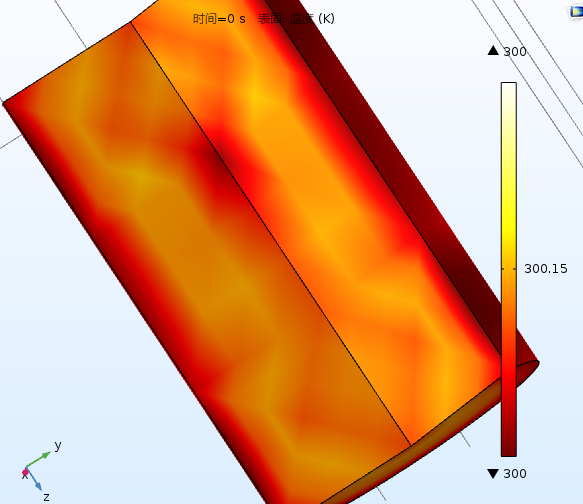
\includegraphics[width=0.25\textwidth]{attachments/fig.s1.1.1.png}
		}		
		\subfloat[$I=0.025A$]{\label{fig.s1.1.2}
		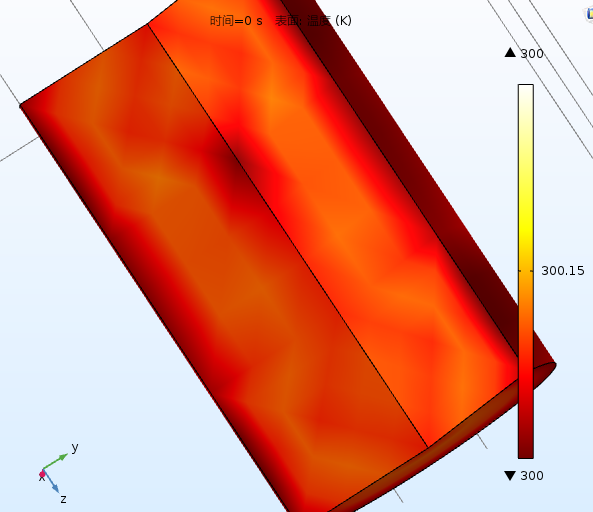
\includegraphics[width=0.25\textwidth]{attachments/fig.s1.1.2.png}
		}

		\subfloat[$I=0.030A$]{\label{fig.s1.1.3}
		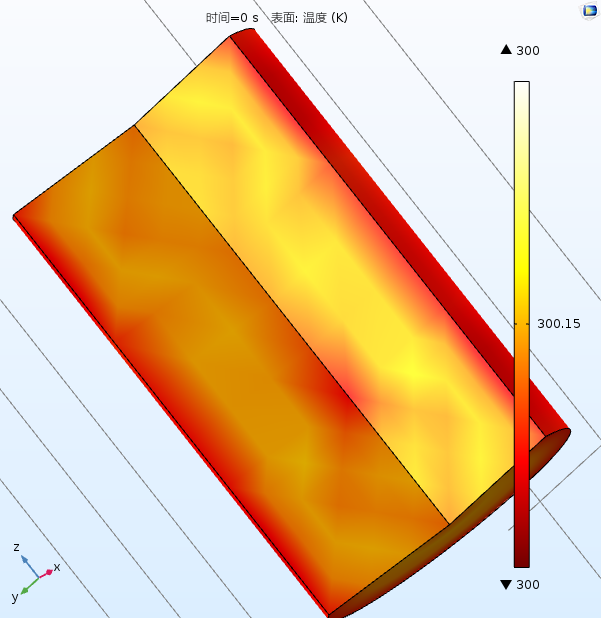
\includegraphics[width=0.25\textwidth]{attachments/fig.s1.1.3.png}
		}
		\subfloat[$I=0.035A$]{\label{fig.s1.1.4}
		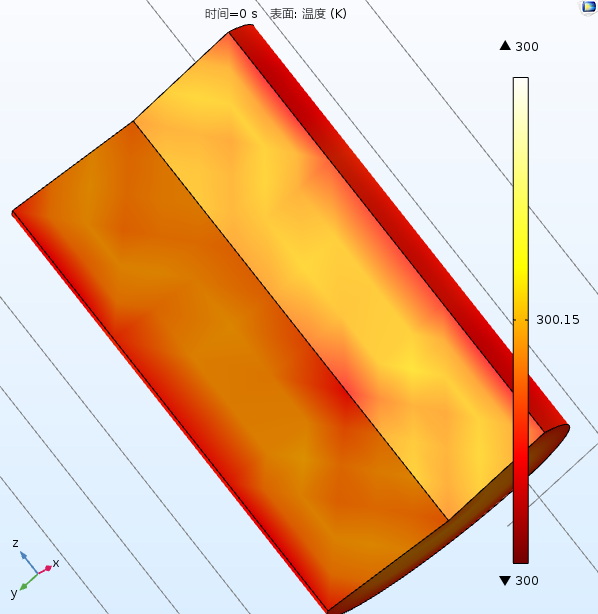
\includegraphics[width=0.25\textwidth]{attachments/fig.s1.1.4.png}
		}
		\subfloat[$I=0.040A$]{\label{fig.s1.1.5}
		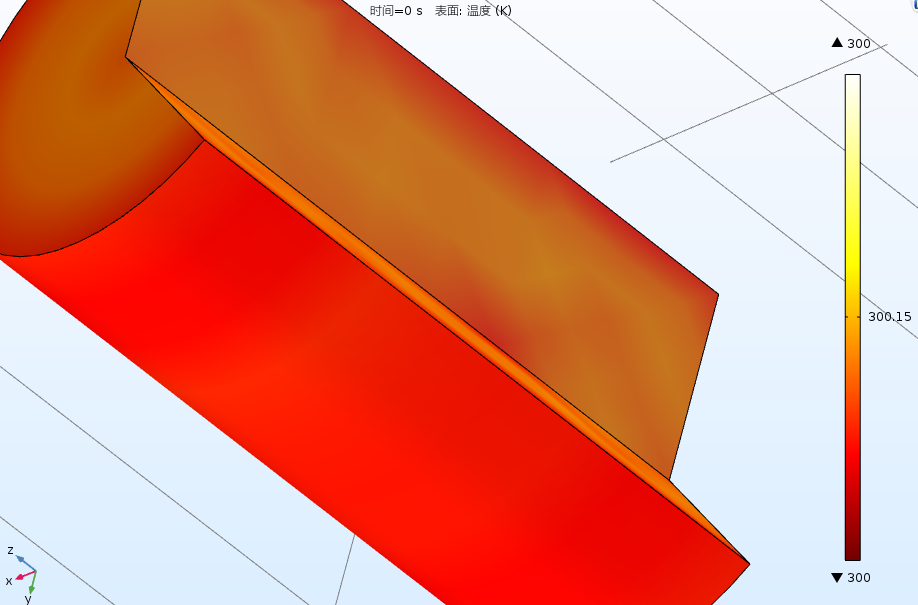
\includegraphics[width=0.25\textwidth]{attachments/fig.s1.1.5.png}
		}
		\caption{\textbf{Temperature field distribution of the ideal resistor model.}}
		\label{fig.s1.1}
	\end{figure*}
	
    \begin{figure*}[htbp]
		\centering
		\subfloat[$I=0.020A$]{\label{fig.s1.2.1}
		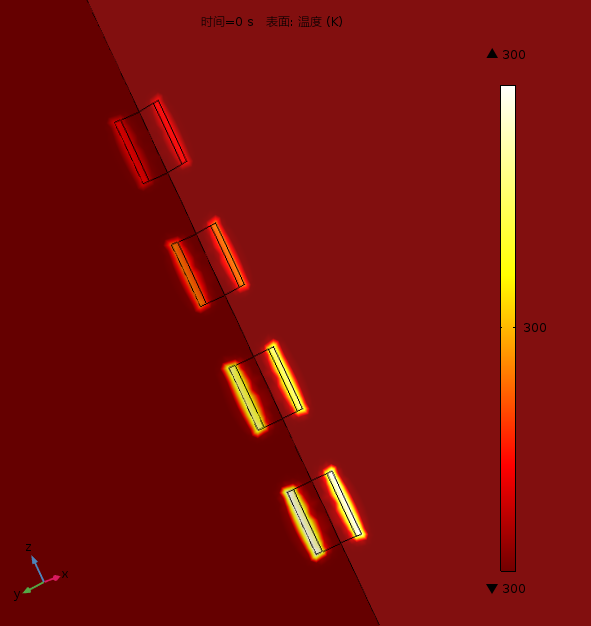
\includegraphics[width=0.25\textwidth]{attachments/fig.s1.2.1.png}
		}		
		\subfloat[$I=0.025A$]{\label{fig.s1.2.2}
		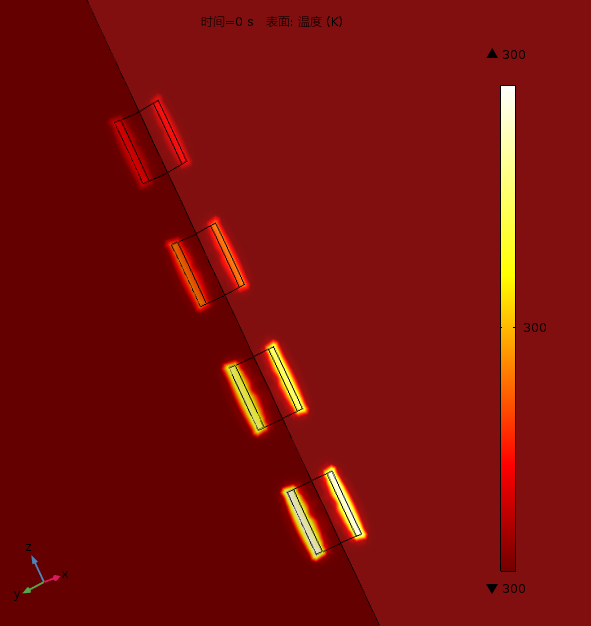
\includegraphics[width=0.25\textwidth]{attachments/fig.s1.2.2.png}
		}

		\subfloat[$I=0.030A$]{\label{fig.s1.2.3}
		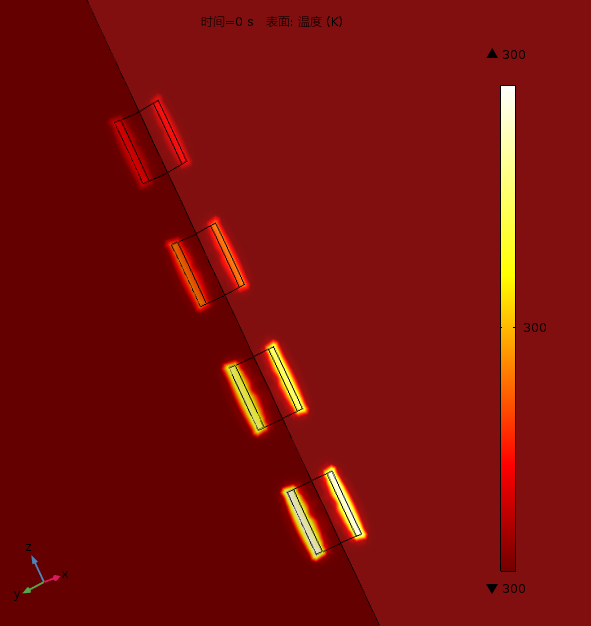
\includegraphics[width=0.25\textwidth]{attachments/fig.s1.2.3.png}
		}
		\subfloat[$I=0.035A$]{\label{fig.s1.2.4}
		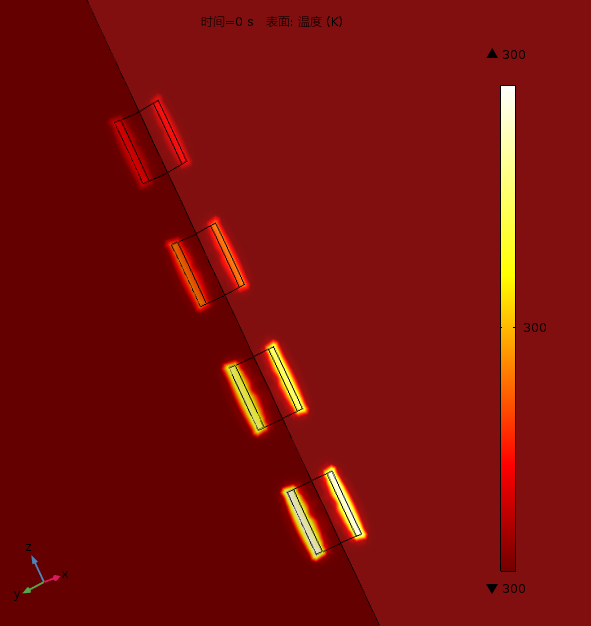
\includegraphics[width=0.25\textwidth]{attachments/fig.s1.2.4.png}
		}
		\subfloat[$I=0.040A$]{\label{fig.s1.2.5}
		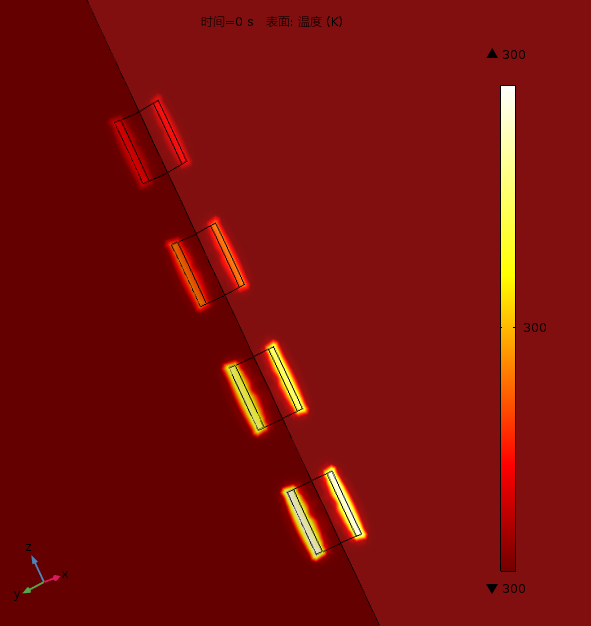
\includegraphics[width=0.25\textwidth]{attachments/fig.s1.2.5.png}
		}
		\caption{\textbf{Temperature field distribution of the complex resistor model.}}
		\label{fig.s1.2}
	\end{figure*}


    \subsection{Question}
        \subsubsection{What are Dirichlet condition, Neumann condition and Robin condition? Which of them can COMSOL deal with?}
        \begin{enumerate}[label=\arabic*.]
            \item Dirichlet condition: The temperature of the boundary is fixed ($u_{|s} = u_0(r, t)$).
            \item Neumann condition: The temperature of the boundary is determined by the heat flux ($\frac{\partial u}{\partial n}_{|s} = \frac{q(r, t)}{k}$).
            \item Robin condition: The temperature of the boundary is determined by Newton's cooling law ($(\frac{\partial u}{\partial n}+hu)_{|s} = hu_0(r, t)$).
            \item COMSOL is capable of dealing with all three types of conditions.
        \end{enumerate}
        \subsubsection{Improve the performance of the model}
        \begin{enumerate}[label=\arabic*.]
            \item Refine the structure of the model: For instance, the model of the resistor can be further refined by adding the electrodes and the insulating layer and so on.
            \item Ascertain the accurate values of the properties of materials: Accurate values of the properties of materials should be carefully measured in real-world experiments rather than using empirical values.
            \item Increase the complexity of computation: A finer mesh and greater number of sampling points, if available, may increase the accuracy of the model.
        \end{enumerate}

% %end---------------------Exp.1---------------------------%

% %begin---------------------Exp.2---------------------------%

\section{Exp.2 Plate model}

    \subsection{Main parameters}
    Parameters including the resistance value of the heater($r /Omega$), the heating voltage($U/V$), 
    default Area correction factor($A$), and the heat exchange coefficient($H$) are shown in Tab. \ref{tab.s2.1}. 
    Values of properties of different materials adapted in the simulation experiment are summarized in Tab. \ref{tab.s2.2}. 
    $C_p (J/kg\cdot K)$: Specific heat capacity at constant pressure; $\rho (kg/m^3)$: Density; $k (W/m\cdot K)$: Thermal conductivity.
    
    \begin{table}[htbp]
        \centering
        \caption{\textbf{Parameters}}
        \label{tab.s2.1}
            \begin{tabular}{ll}
                \toprule
                Item &parameters  \\
                \midrule
                Heating voltage $U$ &$17.0V$ \\
                Resistance $R$ &$110 /Omega$ \\
                Area correction factor$A$ &0.85 \\
                Heat exchange coefficient$H$ &50 \\
                \bottomrule
            \end{tabular}
    \end{table}	

    \begin{table}[htbp]
        \centering
        \caption{\textbf{Material properties}}
        \label{tab.s2.2}
            \begin{tabular}{llll}
                \toprule
                Material &$C_p (J/kg\cdot K)$    &$\rho (kg/m^3)$   &$k (W/m\cdot K)$  \\
                \midrule
                Organic glass(Sample) &1333    &1196    &0.168  \\
                Rubber(Sample) &1700    &1374   &0.426  \\
                Aluminum(Heater) &972.5    &2676.8    &67.09  \\
                Film(Heater) &1058    &1533    &33.97  \\
                Frame(Insulator) &920    &1900    &0.90  \\
                Sponge(Insulator) &400    &4200    &0.046  \\
                \bottomrule
            \end{tabular}
    \end{table}	

    \subsection{Supplementary data and figure}
    \begin{enumerate}[label=\arabic*.]
        \item Fig. \ref{fig.s2.1}: Temperature field distribution of the four models.
        \item Fig. \ref{fig.s2.2}: Change the area correction factor $A$ for Model 1. 
    \end{enumerate}
	
    \begin{figure*}[htbp]
		\centering
		\subfloat[Mod.1 Organic glass]{\label{fig.s2.1.1}
		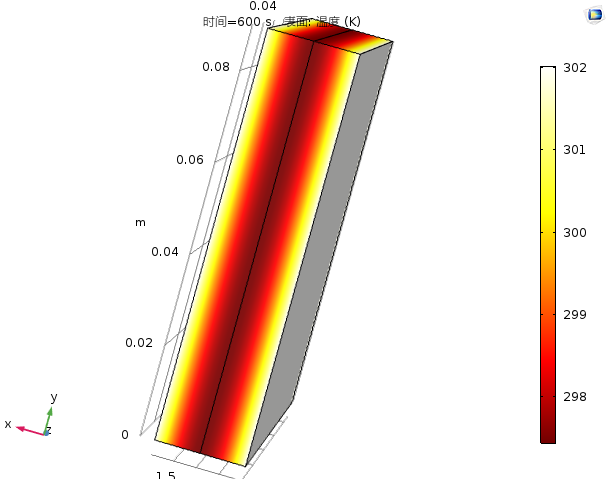
\includegraphics[width=0.25\textwidth]{attachments/fig.s2.1.1.png}
		}		
		\subfloat[Mod.1 Rubber]{\label{fig.s2.1.2}
		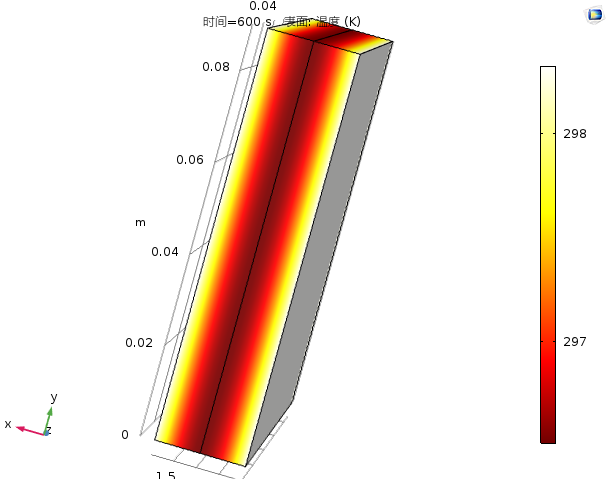
\includegraphics[width=0.25\textwidth]{attachments/fig.s2.1.2.png}
		}
		\subfloat[Mod.2 Organic glass]{\label{fig.s2.2.1}
		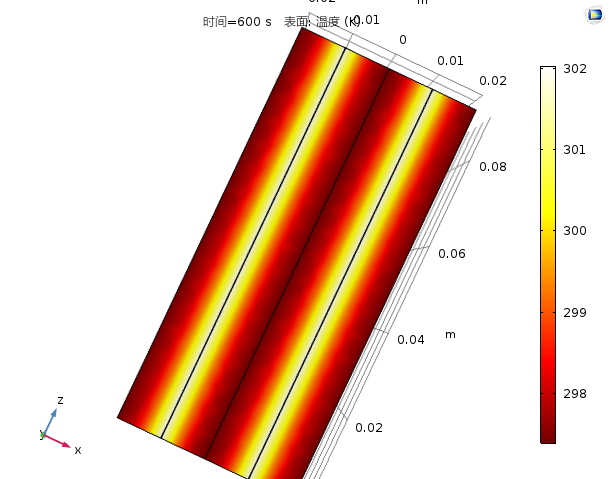
\includegraphics[width=0.25\textwidth]{attachments/fig.s2.2.1.png}
		}		
		\subfloat[Mod.2 Rubber]{\label{fig.s2.2.2}
		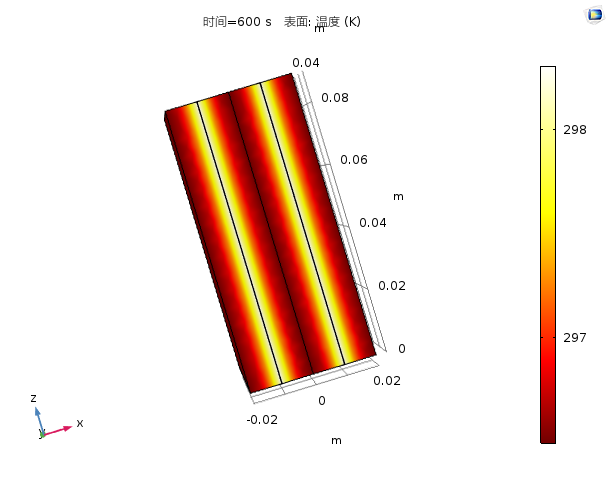
\includegraphics[width=0.25\textwidth]{attachments/fig.s2.2.2.png}
		}

		\subfloat[Mod.3 Organic glass]{\label{fig.s2.3.1}
		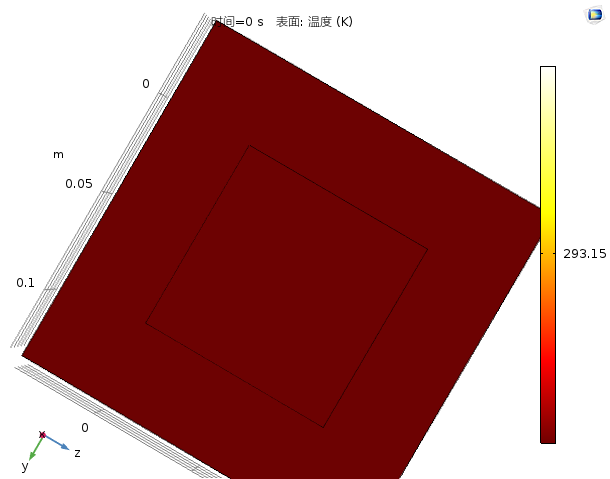
\includegraphics[width=0.25\textwidth]{attachments/fig.s2.3.1.png}
		}		
		\subfloat[Mod.3 Rubber]{\label{fig.s2.3.2}
		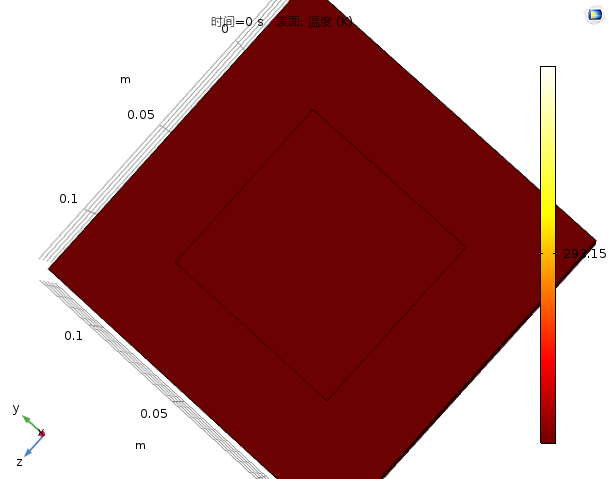
\includegraphics[width=0.25\textwidth]{attachments/fig.s2.3.2.png}
		}
		\subfloat[Mod.4 Organic glass]{\label{fig.s2.4.1}
		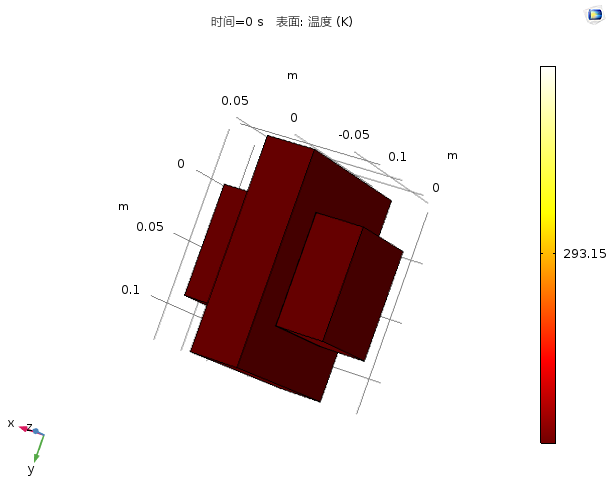
\includegraphics[width=0.25\textwidth]{attachments/fig.s2.4.1.png}
		}		
		\subfloat[Mod.4 Rubber]{\label{fig.s2.4.2}
		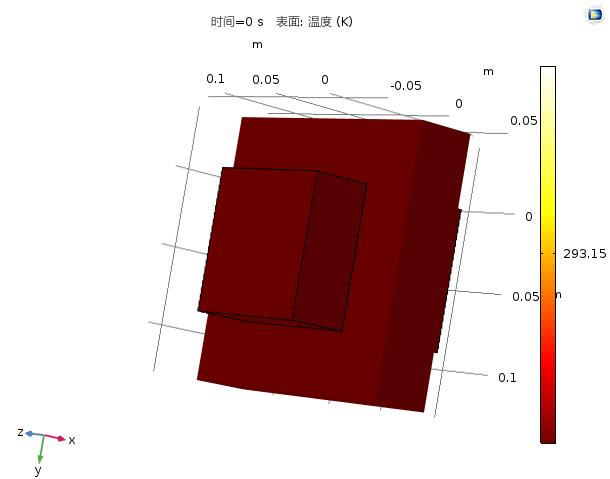
\includegraphics[width=0.25\textwidth]{attachments/fig.s2.4.2.png}
		}
		\caption{\textbf{Temperature field distribution of the ideal resistor model.}}
		\label{fig.s2.1}
	\end{figure*}

    \begin{figure*}[htbp]
		\centering
		\subfloat[Mod.1 $A=0.60$]{\label{fig.s2.5.1}
		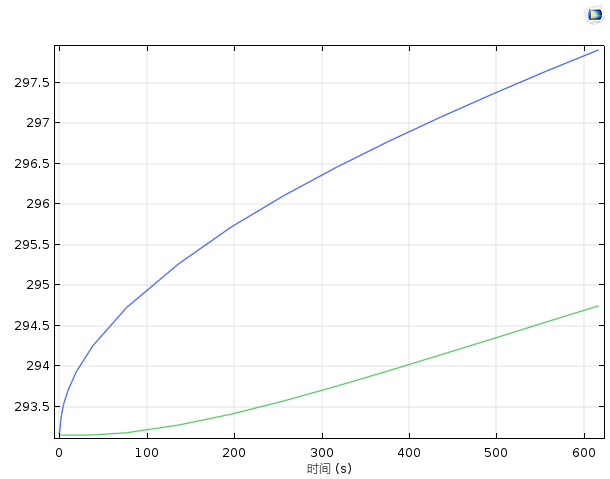
\includegraphics[width=0.4\textwidth]{attachments/fig.s2.5.1.png}
		}		
		\subfloat[Mod.1 $A=0.85$]{\label{fig.s2.5.2}
		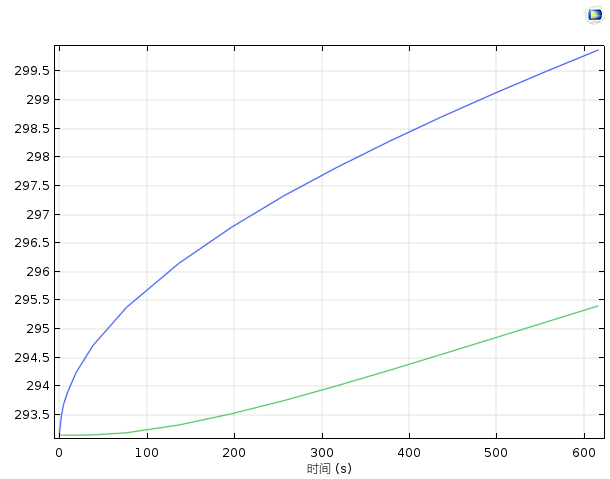
\includegraphics[width=0.4\textwidth]{attachments/fig.s2.5.2.png}
		}
		\caption{\textbf{Change the area correction factor $A$ for Model 1}}
		\label{fig.s2.2}
	\end{figure*}

    \subsection{Question}
        \subsubsection{Why to set the area correction factor $\boldsymbol{A}$?}
        The area correction factor is used to correct the area of the heater to eliminate the edge effect. 
        In the four-sample model, the heat flux $\boldsymbol{q}$ can be expressed as:
        \begin{equation}
            \boldsymbol{q} = \frac{U^2}{2Fr}
        \end{equation}
        where $F=AS$ is the heating area after correction of the edge effect, $A$ is the area correction factor, 
        and $S$ is the actual area of the heater.

        $\boldsymbol{A}$ sometimes need to be adjusted empirically as illustrated in Fig. \ref{fig.s2.2}. 
        We found that if the area correction factor is set to 0.6, the results are more approximate to the results of real-world experiment.

%end---------------------Exp.2---------------------------%


\section{Data and code availability}
Data and code are available at \url{https://github.com/Jeg-Vet/SYSU-PHY-EXP/tree/main/}

\end{document}